%Texlive-full Version 3.141592-1.40.3 (Web2C 7.5.6)
%Kile Version 2.0.83

%File associated : SoFa_Logo.ps
\documentclass[a4paper,10pt]{article}
\usepackage[utf8x]{inputenc}

\usepackage{lmodern}
\usepackage[a4paper]{geometry}
%\usepackage[frenchb]{babel}
\usepackage{graphicx}
\usepackage{hyperref}

\usepackage{pstricks}
\usepackage{pst-node}
%\usepackage{wrapfig}
\usepackage{amsmath}
\usepackage{amssymb}

\usepackage{listings}
\lstset{language=C++,basicstyle=\scriptsize \color{green},identifierstyle=\color{orange},keywordstyle=[1]\color{blue},columns=fullflexible}

\begin{document}
%%%%%%%%%%%%%%%%%%   LOGO  %%%%%%%%%%%%%%%%%%%%%%%%%
\begin{center}
\rput(6,1.5){\href{http://www.sofa-framework.org/}{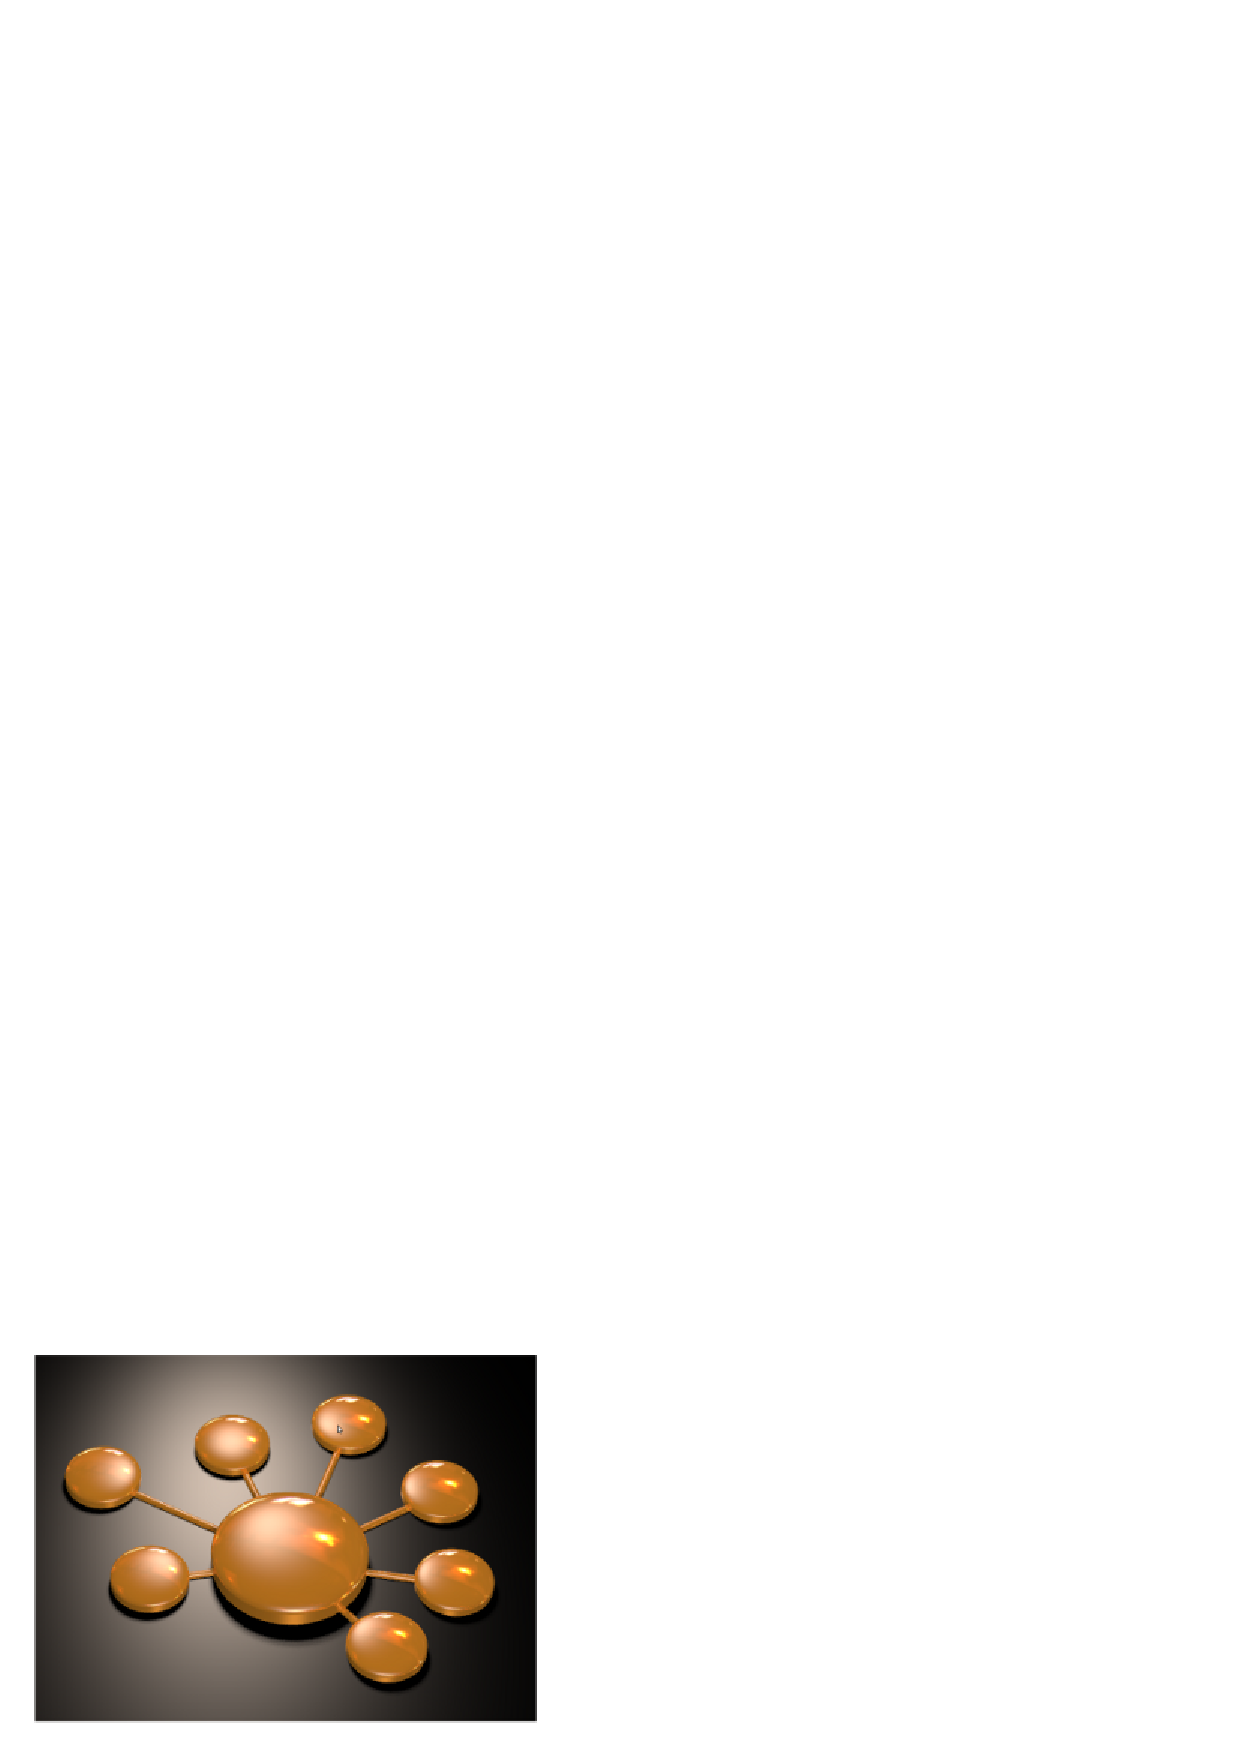
\includegraphics[scale=0.3]{SoFa_Logo}}}
\rput(-4,1.5){\href{http://www.sofa-framework.org/}{
		\begin{tabular}{l}
		\resizebox{4cm}{0.6cm}{SOFA} \\ 
		\resizebox{6cm}{0.3cm}{Simulation Open Framework Architecture}
		\end{tabular}
		}
	    }
\end{center}
%%%%%%%%%%%%%%%%%%   LOGO  %%%%%%%%%%%%%%%%%%%%%%%%%

%%%%%%%%%%%%%%%%%% DOCUMENT TITLE %%%%%%%%%%%%%%%%%%%%%%%%%
%\chapter{Mapping} %\section{Rigid Mapping} 
\vspace{1.5cm}
\begin{center}\resizebox{8cm}{0.5cm}{Deformable On Rigid Mapping}\end{center}
%%%%%%%%%%%%%%%%%% DOCUMENT TITLE %%%%%%%%%%%%%%%%%%%%%%%%%

%%%%%%%%%%%%%%%%%%%%%%%%%%%%%%%%%%%%%%%%%%%%%%%%%%%%%%%%%%%%%%%%%%%%%%%%%%%%%%%%%%%%%%%%%
%=======================================================================================%
%%%%%%%%%%%%%%%%%%%%%%%%%%%%%%%%%%%%%%%%%%%%%%%%%%%%%%%%%%%%%%%%%%%%%%%%%%%%%%%%%%%%%%%%%
\paragraph{Motivation: } Rigid bodies kinematics and dynamics are already modeled in Sofa, but in reality mechanical objects could be a non perfect rigid. It suggest to creat a rigid model allowing a bit of deformation. The idea for computation is the same one of Rigid Mapping combining with a deformable local frame.
\begin{center}
\begin{pspicture}(-7,-1)(7,2)
%\psline(-7,-1)(7,2)
\rput(-2.5,1.5){\Rnode{RigidF}{\Huge{Rigid Frame}}}
\rput(-5.5,1.1){\Rnode{DeformF}{\small{Deformable Frame}}}
\rput(-2.5,0){\ovalnode{Local}{Local Frame}}
\rput(4,0){\Rnode{Global}{\psframebox{Global Frame}}}
\ncarc[arcangle=-20]{->}{Global}{Local} 
\ncarc[arcangle=-20]{->}{Local}{Global}
\ncline{->}{RigidF}{Local} 
\ncline{->}{DeformF}{Local}
\end{pspicture}
\end{center}
  

\paragraph{Definitions: }
\begin{itemize}
 \item Model Behaviour Rigid : Position and orientation (quaternion) of the center(s) of mass.
 \item Model Colision Rigid : A set of particles used for computing the colision with other objects.
 \item Model Deformable Rigid : A set of particle used for modeling the deformation.
\end{itemize}
It is needed to well understand the Rigid Mapping for good understanding the Deformable On Rigid Mapping. 
\paragraph{Computation: } Generalized from the perfect Rigid model, the Deformable Rigid model is more complicated, but consist also updating the particles position, velocity and computing the effect of the external forces. The Deformable Rigid has tree frame of reference : a global frame and a local frame like in the perfect Rigid, a further local frame. The unique aim of the added frame is modeling the deformation, so this frame will be fixed in relation to the global frame and don't have any rotation or translation. To find the particles positions, the center position must be found at first. The other ones will be found locally from the deformed system\footnote[1]{$[...]^d$ denote all on the deformable frame}\footnote[2]{$[...]^r$ denote all on the rigid frame} :$OP^r_i=OP^r_0+P^d_0P^d_i$. To find the particles velocities, not only the velocity due to the rigid center motion ($v^r$) must be computed, but also the velocity due to the deformation ($v^d$) must be computed and added. For each particle : $v_i=v^d_i+v^r_i$. External forces applied both to the rigid center and to the deformable model :
\[\sum F_{extern} + \rightarrow 
\left[
\begin{array}{l}
\text{center.} \\
\text{deformable system.}
\end{array}
\right.
\]
\newpage         
%%%%%%%%%%%%%%%%%%%%%%%%%%%%%%%%%%%%%%%%%%%%%%%%%%%%%%%%%%%%%%%%%%%%%%%%%%%%%%%%%%%%%%%%%
%============================           FIGURE        ==================================%
\begin{figure}[h]
\begin{pspicture}(-7,-4)(7,4)
%\psline(-7,-4)(7,4)%%%%%%%%%%%%%%%%%%%%%%%%%%%%%
%%%%%%%%%%% Reference frame Observetor %%%%%%%%%%
\psline[linecolor=red]{->}(-4,-1.5)(-4,0.5)%Z
\psline[linecolor=blue]{->}(-4,-1.5)(-2,-1.5)%Y
\psline[linecolor=green]{->}(-4,-1.5)(-4.6,-2.7)%X
\rput(-4.2,-1.5){O}
%%%%%%%%%%% Reference frame Rigid %%%%%%%%%%%%%%%%%%%%%%%%%%%%%%%%%
\psline[linecolor=red,linewidth=2pt]{->}(3.5,0.5)(4,0.7)%z
\psline[linecolor=blue,linewidth=2pt]{->}(3.5,0.5)(4.2,-0.2)%y
\psline[linecolor=green,linewidth=2pt]{->}(3.5,0.5)(4,1.5)%x
\psccurve[showpoints=true](2.5,2)(2.5,-2)(4.5,-1)(6,2)%Pi P1 P2 P3
\rput(2.2,2.2){$P_i^r$}\rput(2.2,-2.2){$P_1^r$}\rput(4.8,-1){$P_2^r$}\rput(3.3,0.3){\textbf{P}$^r_0$}
%%%%%%%%%%% Reference frame Deformable %%%%%%%%%%
\psline[linecolor=red,linewidth=2pt]{->}(-4,-1.5)(-4,-0.5)%zz
\psline[linecolor=blue,linewidth=2pt]{->}(-4,-1.5)(-3,-1.5)%yy
\psline[linecolor=green,linewidth=2pt]{->}(-4,-1.5)(-4.3,-2.1)%xx
\psccurve[showpoints=true, linestyle=dashed](-6.5,-1.5)(-3.8,-3)(-1.5,-2)(-3.8,0)%PPi PP1 PP2 PP3
\rput(-6.8,-1.5){$P_i^d$}\rput(-3.8,-3.4){$P_1^d$}\rput(-1.2,-2){$P_2^d$}\rput(-3.7,-1.2){\textbf{P}$^d_0$}
%%%%%%%%%%%%%%%%%%% Curve Rigid Surface %%%%%%%%%%%%%%%%%%%%%%%%%%%
%\pnode(3.5,0.5){Po}\pnode(2.5,2){Pi}
%\ncline[linestyle=dotted]{->}{Po}{Pi}\naput{$\vec{r}_i$}
\rput(-5,1){\Rnode{Glob}{\Large{Global Frame}}}
\rput(-2.5,-1.7){\Rnode{Loc2}{\textbf{Deform Frame}}}
\rput{40}(1,2){\Rnode{Loc}{\textbf{Rigid Frame}}}
\ncarc[arcangle=-40]{<->}{Loc}{Glob}\naput{Rotation}
%%%%%%%%%%%%%%%% Rotation axe %%%%%%%%%%%%%%%%%%%%%
\psline[linewidth=4pt]{->}(3.5,0.5)(7,0)%w(t) axe
\psellipticarc{<-}(5.5,0.25)(0.5,1){60}{320}
\rput(6,-0.2){w(t)}
\end{pspicture}
\end{figure}
%============================           FIGURE        ==================================%
%%%%%%%%%%%%%%%%%%%%%%%%%%%%%%%%%%%%%%%%%%%%%%%%%%%%%%%%%%%%%%%%%%%%%%%%%%%%%%%%%%%%%%%%%

\begin{center} To update the particles position :\end{center}
$
\left\|
  \begin{array}{lll}
  \text{Finding  } OP^r_o=LinearPosition; 
  \text{  Finding  } R^{glob}_{loc}=RotationMatrix; \\
  \text{For} (i=1;i<N;i++) \\ \{ \\
    \hspace{1cm} P^r_oP^r_i=R^{glob}_{loc}*P^d_oP^d_i;\\
    \hspace{1cm} OP^r_i=OP^r_o+P^r_oP^r_i;\\
    \} 
  \end{array}
\right.
$

\begin{center}To update the particles velocity : \end{center}
$
\left\|
  \begin{array}{lll}
  \text{Finding  } V^r_{P_O}=LinearVelocity;
  \text{   Finding  } w^r_{Po}=AngularVelocity; \\
  \text{For} (i=1;i<N;i++) \\ \{ \\
    \hspace{1cm} V^r_i= V^r_{P_O} - P^r_oP^r_i \wedge w^r_{Po} ;\\
    \hspace{1cm} R=RotationMatrix \text{  ;  } V^d_i=R*V_{P^d_i};\\
    \hspace{1cm} V_i= V^r_i + V^d_i; \\
    \} 
  \end{array}
\right.
$
\begin{center}To compute the reponse of the external forces:\end{center}    
$
\left\|
  \begin{array}{lll}
  \text{For} (i=1;i<N;i++) \\ \{ \\
    \hspace{1cm} F_{exter}+=f_i;\\
    \hspace{1cm} Torque+=P_oP_i  \wedge  f_i\\
    \hspace{1cm} R=\left[ RotationMatrix \right]^{-1} \text{  ;  } F_{P^d_i}=R*f_i;\\
    \} \\
  \text{Update } LinearForceCenter=F_{exter}; \\
  \text{Update } AngularForceCenter=Torque; 
  \end{array}
\right.
$
\newpage
\paragraph{Implementated code in Sofa: }These algorithms are implemented in Sofa by the following methods : \\
To update the particles position :
\begin{lstlisting}
template <class BasicMapping>
void DeformableOnRigidFrameMapping<BasicMapping>::apply(typename Out::VecCoord & out,
                                                                const typename In::VecCoord & inDeformed, 
                                                                const typename InRoot::VecCoord * inRigid)
\end{lstlisting}
To update the particles velocity :
\begin{lstlisting}
template <class BasicMapping>
void DeformableOnRigidFrameMapping<BasicMapping>::applyJ(typename Out::VecDeriv &  out,
								 const typename In::VecDeriv & inDeformed,
								 const typename InRoot::VecDeriv* inRigid)
\end{lstlisting}
To compute the external forces soliciting to center :
\begin{lstlisting}
template <class BasicMapping>
void DeformableOnRigidFrameMapping<BasicMapping>::applyJT(typename In::VecConst & out,
								  const typename Out::VecConst & in,
								  typename InRoot::VecConst*  outroot)

\end{lstlisting}

\paragraph{Sofa Keyword: } Rigid Mapping, Deformable on Rigid Frame Mapping.


						      %%%%%%%%%%%%%%%%%%%%%%%%%%  Writer %%%%%%%%%%%%%%%%%%%%%%%%
						      \begin{flushright}
						      Document written by \\
						      \href{mailto:chi-thanh.nguyen@inria.fr}{{\textbf {Chi Thanh NGUYEN}}} \\
						      INRIA Lille
						      \end{flushright}
						      %%%%%%%%%%%%%%%%%%%%%%%%%%  Writer %%%%%%%%%%%%%%%%%%%%%%%%

\end{document}
